\documentclass[12pt, 
hyperref={colorlinks=true, linkcolor=BlueViolet, urlcolor=BlueViolet},dvipsnames]{beamer}
\usetheme{default} 

\setbeamertemplate{navigation symbols}{} %gets rid of navigation symbols
\setbeamertemplate{footline}{} %gets rid of bottom navigation bars
\setbeamertemplate{footline}[page number]{} %use this for page numbers

\setbeamertemplate{footline}{%
  \raisebox{5pt}{\makebox[\paperwidth]{\hfill\makebox[10pt]{\scriptsize\insertframenumber~~}}}}

\setbeamertemplate{itemize items}[circle] %round bullet points
\setlength\parskip{10pt} % white space between paragraphs

\usepackage{wrapfig}
\usepackage{subfig}
\usepackage{setspace}
\usepackage{enumerate}
\usepackage{graphicx}
\usepackage{amsmath}
\usepackage{amsfonts}
\usepackage{amssymb}
\usepackage{amsthm}
\usepackage[UKenglish]{isodate}
\usepackage{verbatim}
\usepackage{xcolor}
\cleanlookdateon

% new amber color
\definecolor{amber}{rgb}{1.0, 0.75, 0.0}


% the preamble
\title{Lecture 9: Cluster computing}
\author{Brian Williamson}
\institute{BIOST 561: Computational Skills For Biostatistics I}
\date{29 May 2019}

% Start the document
\begin{document}
% The title page
\begin{frame}
\titlepage
\end{frame}

% motivation
\section{Introduction}
\begin{frame}
\frametitle{Motivation}
We are often interested in \textcolor{cyan}{large-scale} computing: \vspace{-0.3cm} \pause
\begin{itemize}
\item simulation studies (e.g., lecture 4) \pause
\item intensive data analyses (e.g., \href{https://www.nejm.org/doi/full/10.1056/nejmoa1702747}{air pollution and mortality}) \pause
\end{itemize}

In Lecture 8, you learned how to compute without \texttt{R}. 

Today, you'll learn how to transfer those skills to computing on a \textcolor{ForestGreen}{cluster}.

\end{frame}

\begin{frame}
\frametitle{Examples from my research}
\textcolor{cyan}{Large-scale} simulation studies: \vspace{-0.3cm} \pause
\begin{itemize}
\item proof-of-concept examples \pause
\item showcase \textcolor{ForestGreen}{operating characteristics} of proposed method
\end{itemize} \pause

\begin{center}
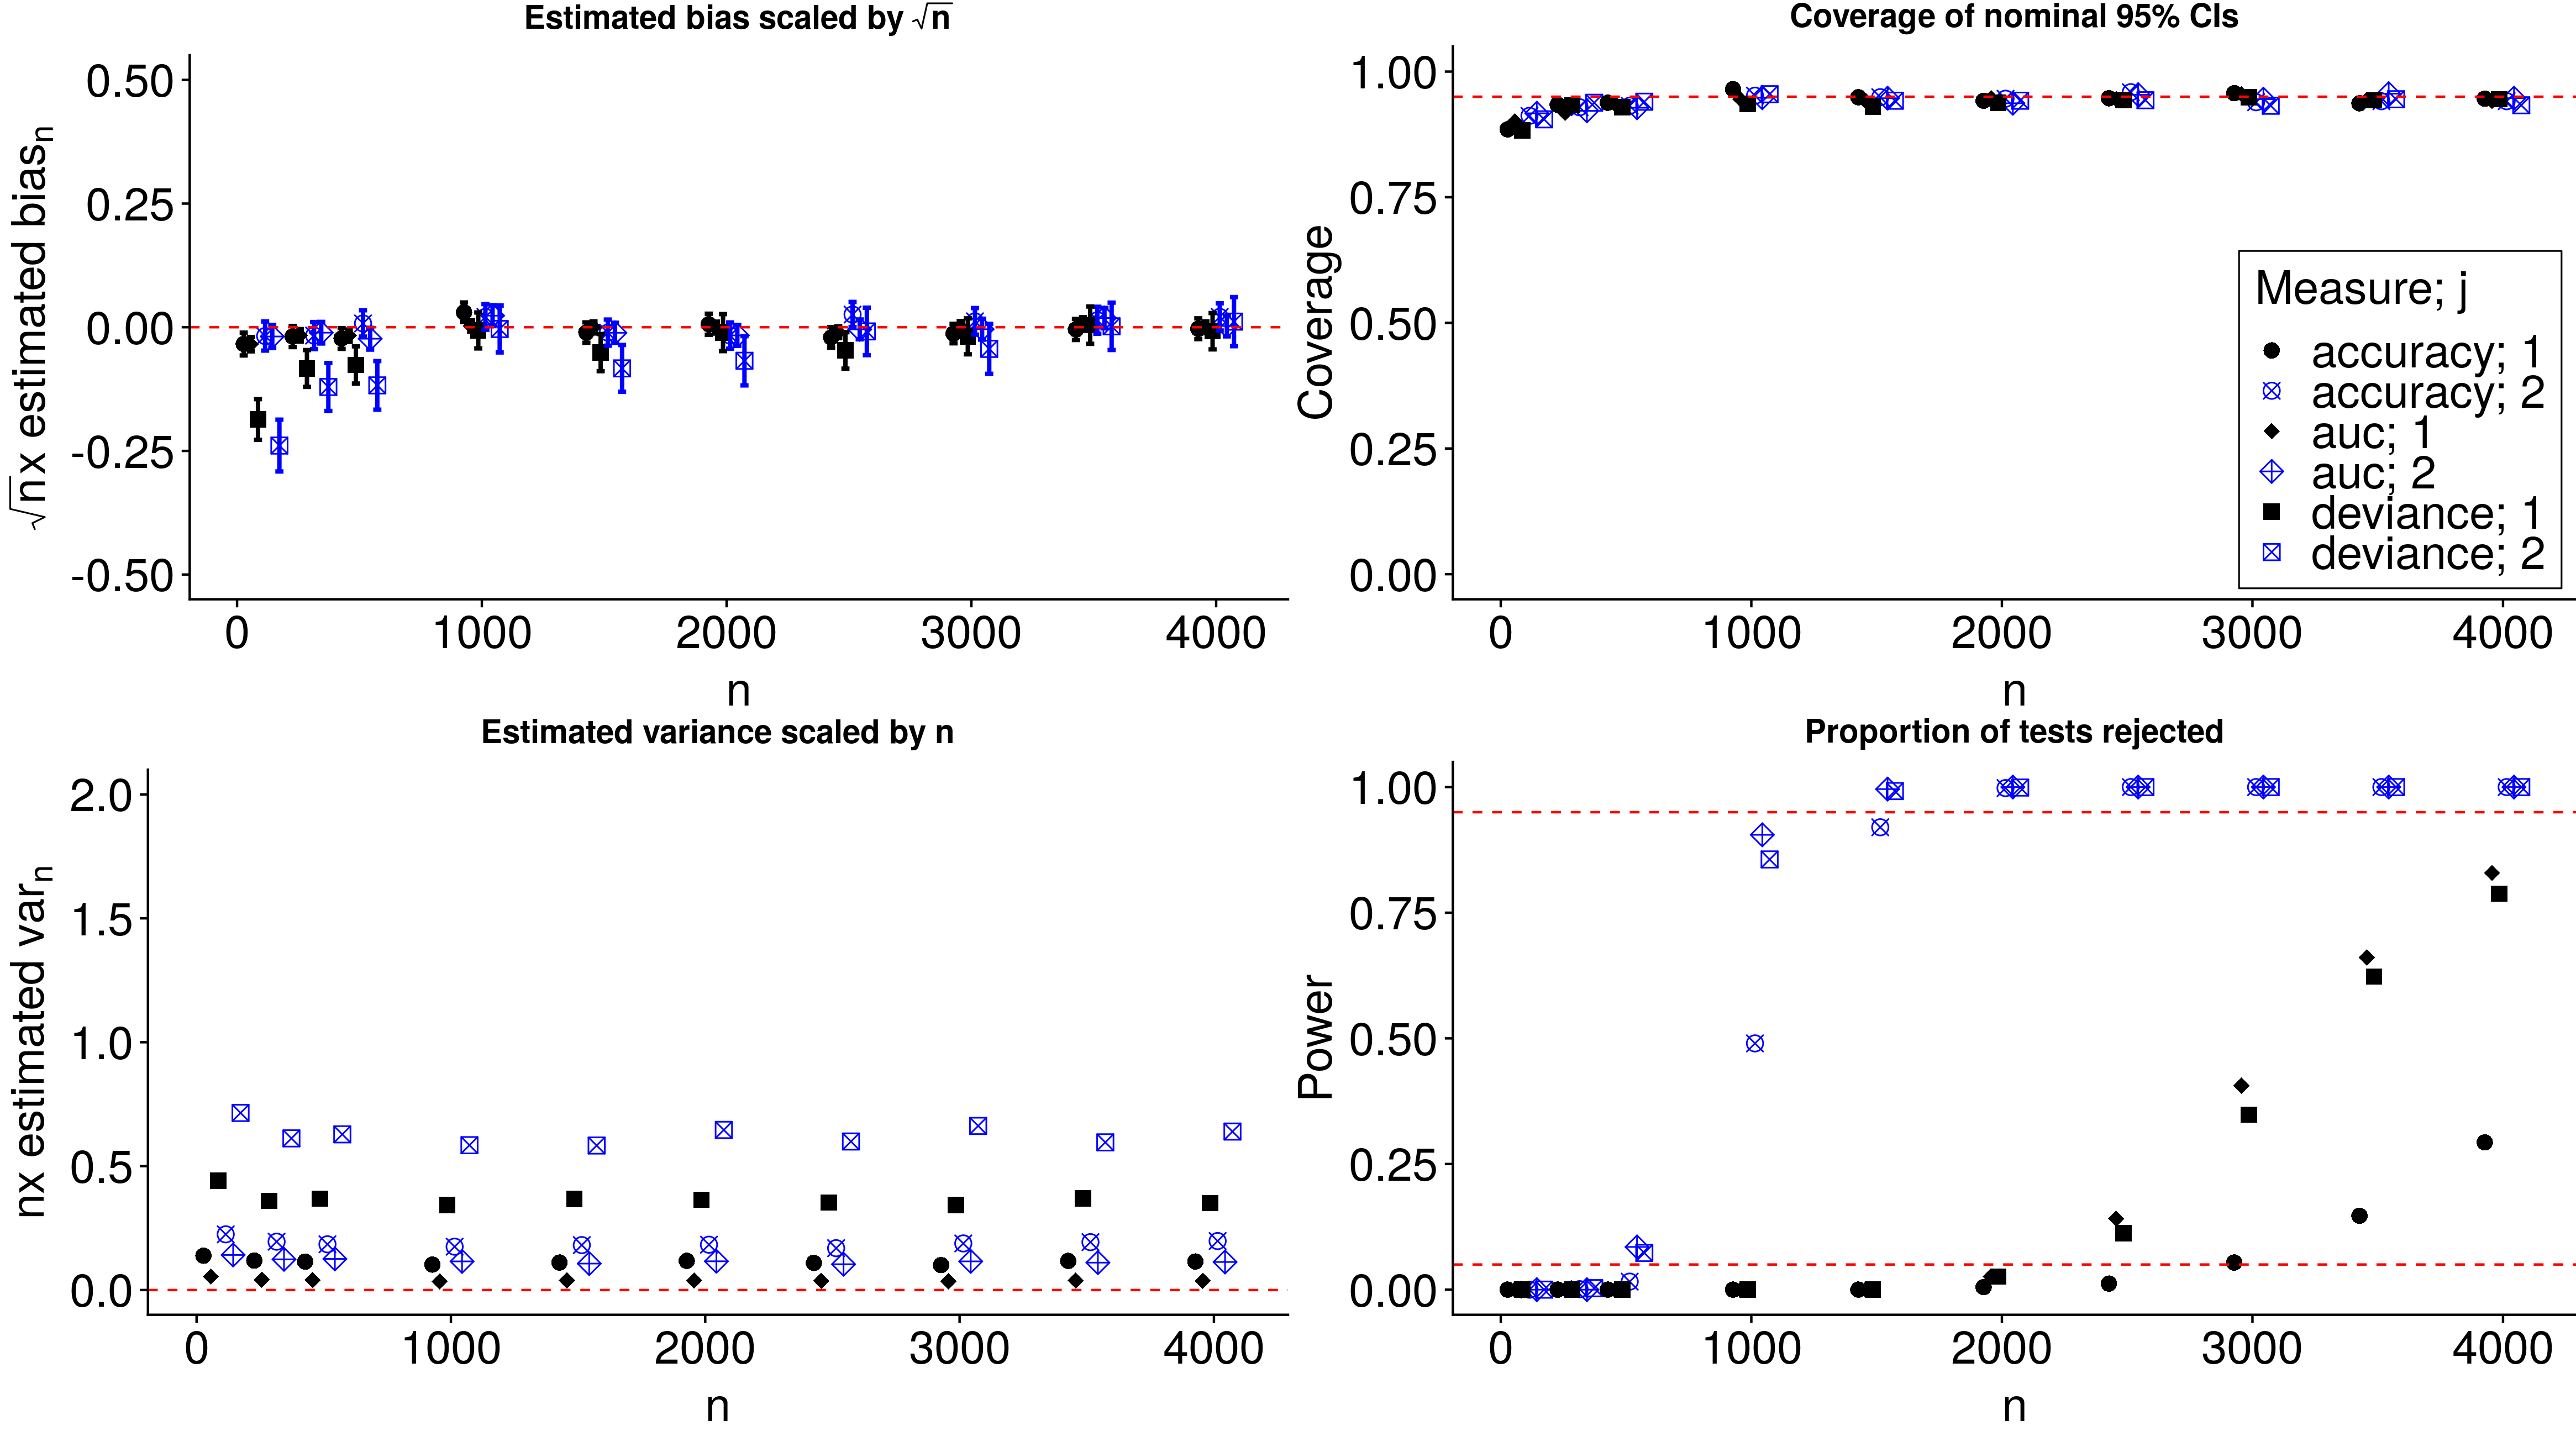
\includegraphics[width = 1\textwidth]{plots/bivariate_loss_performance_deviance_accuracy_auc.png}
\end{center}
\end{frame}

\begin{frame}
\frametitle{Examples from my research}
\textcolor{BurntOrange}{Data analysis}: \vspace{-0.3cm} \pause
\begin{itemize}
\item fit a time-consuming estimator \pause
\item cross-validation? \pause
\item memory-intensive computations? \pause
\end{itemize}

\begin{center}
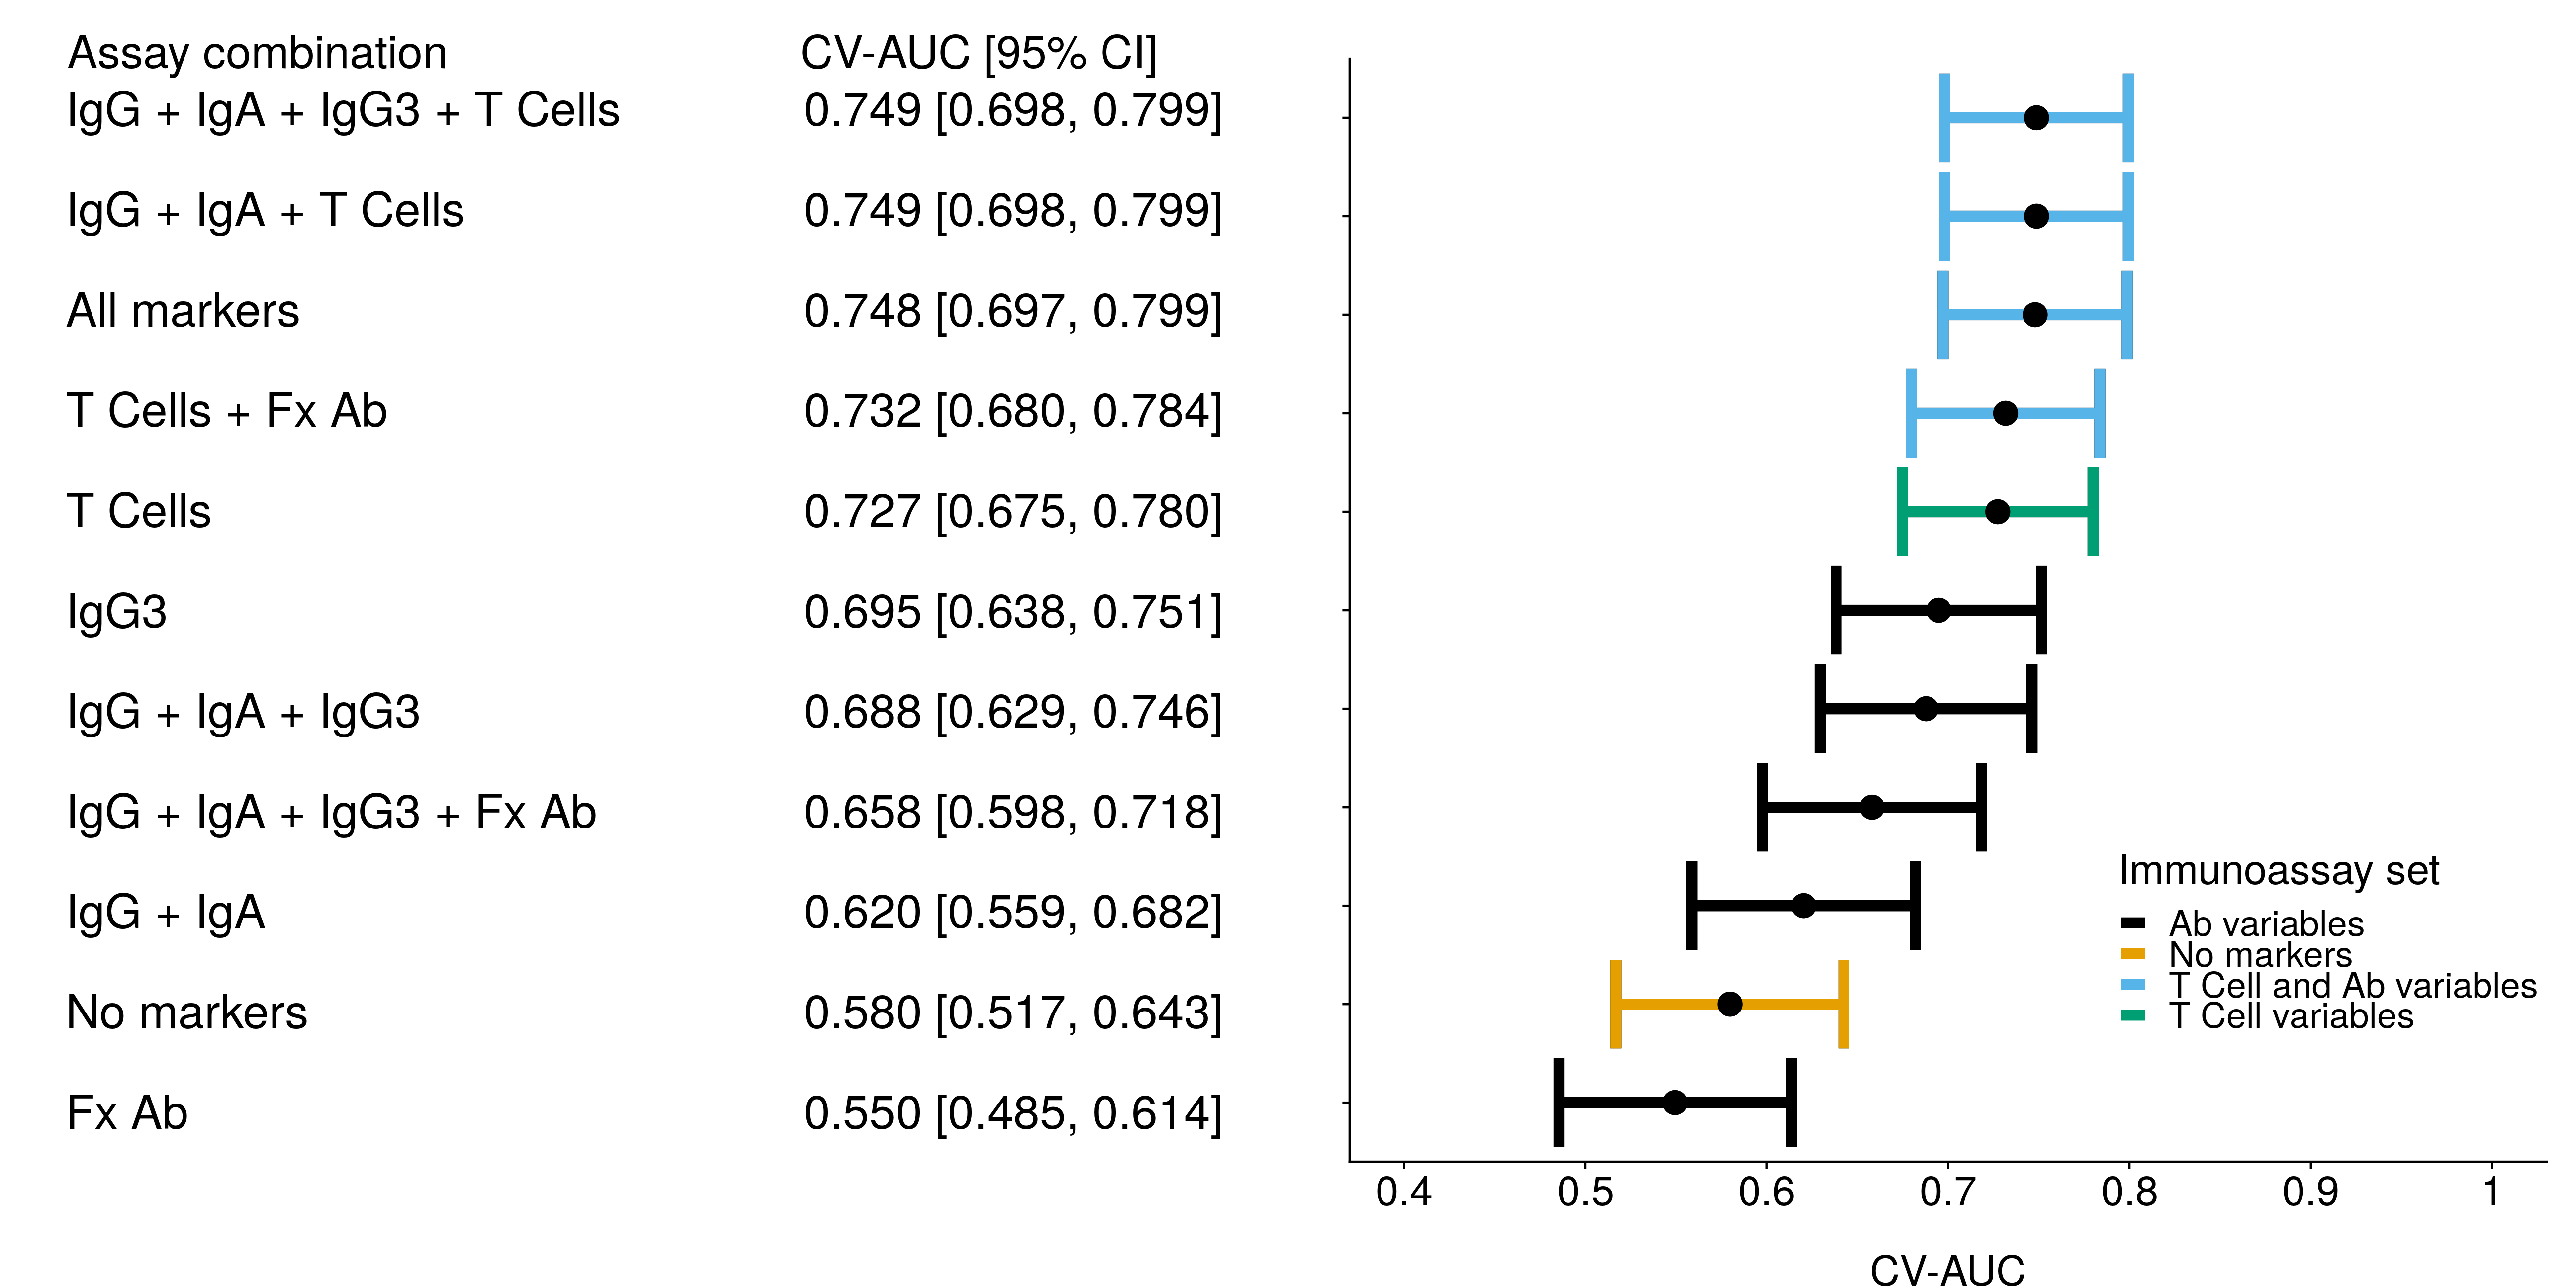
\includegraphics[width = 1\textwidth]{plots/cv_auc_forest_plot_sl.png}
\end{center}
\end{frame}

\begin{frame}
\frametitle{The problem}
How do I run\vspace{-0.3cm} \pause
\begin{itemize}
\item \textcolor{blue}{many} \pause
\item potentially \textcolor{red}{time-consuming} \pause
\item or \textcolor{red}{memory-intensive} \pause
\end{itemize}
analyses without \pause keeping an R session open (\textcolor{red}{for the duration!}) \pause \textcolor{red}{on my personal machine}?
\end{frame}

\begin{frame}
\frametitle{The solution}
Cluster computers provide a solution! \pause

Cluster computers: \vspace{-0.3cm} \pause
\begin{itemize}
\item allow you to \textcolor{blue}{submit multiple \textbf{jobs}${}^*$ at once} \pause
\item can \textcolor{blue}{schedule jobs for you} \pause
\item are \textcolor{blue}{optimized} for high-performance computing (HPC) \pause
\end{itemize}

{\small ${}^*$: we will discuss this further!}
\end{frame}

\begin{frame}
\frametitle{Running example: robust standard errors (SEs)}

Consider a sample of $n$ observations generated iid according to
\begin{align*}
X \sim & \ N(0, 1), \\
u \sim & \ N(0, 1), \text{ independent of $X$}; \\
Y \mid X, u =& \ \beta_0 + \beta_1 X + \epsilon, \text{ where } \\
\epsilon =& \ \lvert X \rvert u.
\end{align*}

Questions: can we use \vspace{-0.3cm}
\begin{enumerate}
\item linear regression to estimate $\beta_1$? \pause \textcolor{blue}{Yes!} \pause
\item model-based standard errors to estimate $sd(\beta_1)$? \pause \textcolor{red}{No!} \pause
\item robust standard errors to estimate $sd(\beta_1)$? \pause \textcolor{blue}{Yes!}
\end{enumerate}
\end{frame}

\begin{frame}
\frametitle{Running example: robust SEs}
Goals: \vspace{-0.3cm}  \pause
\begin{itemize}
\item compare model-based to robust SEs \pause
\item do this without using our own computers \pause
\end{itemize}

We will use the cluster to do this!
\end{frame}

% section 1: coding in a cluster-friendly way
\section{Coding for the cluster}
\begin{frame}
\frametitle{}
\begin{center}
{\large \textbf{Part I: coding for the cluster}}
\end{center}
\end{frame}

\begin{frame}
\frametitle{Coding for the cluster}
Before moving to the cluster, we need to code differently: \vspace{-0.3cm} \pause
\begin{itemize}
\item modular code \pause (\textcolor{cyan}{easy debugging}) \pause
\item setting seeds \pause (\textcolor{ForestGreen}{reproducible results}) \pause
\item saving output \pause (\textcolor{BurntOrange}{for results!})
\end{itemize}

The \texttt{simulator} (Lecture 4) makes this easy: \vspace{-0.3cm} \pause
\begin{itemize}
\item forces you to code modularly \pause
\item forces you to set a seed \pause
\item forces you to save lots of output \pause
\end{itemize}

A couple of drawbacks: \vspace{-0.3cm} \pause
\begin{itemize}
\item can cause memory leaks \pause
\item sometimes difficult to link to cluster nodes \pause
\end{itemize}

Today, I'll provide an alternative method (this should not always replace the simulator!).
\end{frame}

\begin{frame}
\frametitle{Coding for the cluster: modular code}
Modular code: each file has a single task \pause

Your turn!

Go to the \texttt{code} subdirectory. Then answer these questions \textbf{with a partner}: \vspace{-0.3cm}
\begin{enumerate}
\item what does \texttt{do\_one} do? What are its arguments?
\item what does \texttt{generate\_data} do? What are its arguments?
\item Write effective comments in each file so that \textbf{future you} understands each!
\end{enumerate}
\end{frame}

\begin{frame}
\frametitle{Coding for the cluster: modular code}

Answers and Brian's comments (to be posted after class)

\end{frame}

\begin{frame}
\frametitle{Coding for the cluster: setting the seed}

Setting a seed is \textcolor{blue}{vital} if your code involves \vspace{-0.3cm} \pause
\begin{itemize}
\item generating data (e.g., simulation) \pause
\item cross-validation \pause
\item \dots \pause
\end{itemize}
and you want it to be reproducible (you do!). \pause

Things to remember on setting a seed: \vspace{-0.3cm} \pause
\begin{itemize}
\item set seeds in a logical, reproducible way \pause
\item set a \textcolor{cyan}{unique seed} for each job \pause
\end{itemize}

\end{frame}

\begin{frame}
\frametitle{Coding for the cluster: \texttt{\#!} and executables}

In Lecture 8, you learned about \texttt{\#!} and executable files. \pause

\texttt{\#!} (``shebang''): \vspace{-0.3cm} \pause
\begin{itemize}
\item tells your computer where to look for executable file to run your code
\item place at top of file \pause
\end{itemize}

Executables (e.g., \texttt{/bin/sh}): \vspace{-0.3cm} \pause
\begin{itemize}
\item actually run your code
\item other examples: \texttt{/bin/bash}, \texttt{/usr/local/bin/Rscript}, \texttt{/usr/local/bin/python3}
\end{itemize}

\end{frame}

\begin{frame}
\frametitle{Coding for the cluster: saving output}

Running without a graphical user interface (GUI) requires you to pre-specify the output you want to save.

How much/what to save? \pause Depends on what you need! \vspace{-0.3cm} \pause
\begin{itemize}
\item More output: easy debugging, wastes memory/time \pause
\item Think ahead: careful planning can make results tidy/nice \pause
\end{itemize}

This is important regardless of whether or not you use the \texttt{simulator}!

Handy functions for saving output: \texttt{saveRDS}.
\end{frame}

\begin{frame}
\frametitle{Coding for the cluster: saving output}

Your turn!

In the robust SEs example, our goal is to compare model-based to robust SEs. \textbf{With a partner}, answer the following questions: \vspace{-0.3cm}
\begin{enumerate}
\item What output should we save?
\item How should we evaluate performance of the SEs? 
\end{enumerate}
\end{frame}

\begin{frame}
\frametitle{Coding for the cluster: robust SEs}

Check out \texttt{run\_sim\_robust\_se.R} in the \texttt{code} directory!

\end{frame}

\begin{frame}
\frametitle{Coding for the cluster: debugging}

Debugging is hard without a GUI. \pause

Best practices (in my opinion): \vspace{-0.3cm} \pause
\begin{itemize}
\item debug \textbf{everything} on your machine first \pause
\item modular code \pause (isolate bugs) \pause
\item run one job for subset of parameters prior to cluster
\end{itemize}

\end{frame}

\begin{frame}
\frametitle{Coding for the cluster: compiling output}

Check out \texttt{load\_sim\_robust\_se.R} in the \texttt{code} directory!

\end{frame}

% section 2: using the cluster
\section{Using the cluster}
\begin{frame}
\frametitle{}
\begin{center}
{\large \textbf{Part II: using the cluster}}
\end{center}
\end{frame}

\begin{frame}
\frametitle{Using the cluster}
Department resources for HPC${}^*$: \vspace{-0.3cm} \pause
\begin{itemize}
\item \texttt{cox}: 12-core computer \pause (\textcolor{red}{not a cluster}) \pause
\item \texttt{bayes}: compute cluster
\end{itemize}

A cluster consists of: \vspace{-0.3cm} \pause
\begin{itemize}
\item a head node \pause (where you are) \pause
\item compute nodes \pause (where your code gets run) \pause
\item submission system \pause (how your code gets run) \pause
\end{itemize}

{\small ${}^*$other groups have similar resources, e.g., \vspace{-0.3cm}
\begin{itemize}
\item \href{https://itconnect.uw.edu/service/shared-scalable-compute-cluster-for-research-hyak/}{\texttt{hyak}} (managed by UW-IT)
\item \texttt{pearson} (statistical genetics group only)
\item \texttt{gizmo} (Fred Hutchinson Cancer Research Center only)
\item Microsoft Azure, Amazon Web Services (AWS)
\end{itemize}
}
\end{frame}

\begin{frame}
\frametitle{Using the cluster}
\begin{center}
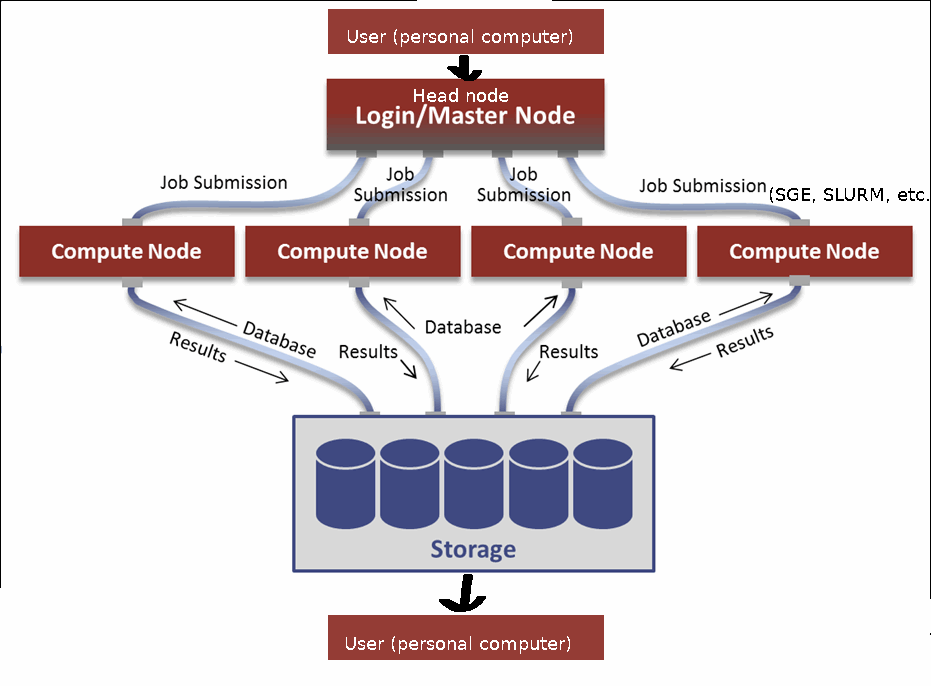
\includegraphics[width = 1\textwidth]{plots/hpc_system.png}
\end{center}
\end{frame}

\begin{frame}
\frametitle{Using the cluster: \texttt{bayes}}
More specifically, \texttt{bayes} \vspace{-0.3cm} \pause
\begin{itemize}
\item has \textcolor{cyan}{4 department-wide} compute nodes, each with \textcolor{blue}{12 cores} \pause
\item uses Sun Grid Engine (\href{https://en.wikipedia.org/wiki/Oracle_Grid_Engine}{SGE}) for submissions \pause
\end{itemize}

Since this is a shared resource, being \textcolor{blue}{nice} is important: \vspace{-0.3cm} \pause
\begin{itemize}
\item don't run simulations on the head node \pause
\item don't flood the cluster \pause
\end{itemize}

We'll practice good habits for being nice as we go along.
\end{frame}



\begin{frame}
\frametitle{Using the cluster: logging in (Windows, incl.~\texttt{box})}
\begin{enumerate}
\item Open TeraTerm [or your favorite secure shell (SSH) client]
\item Enter the address of your favorite cluster, e.g., \texttt{bayes.biostat.washington.edu}
\item Make sure that the ``New connection'' window is filled out as in the figure, except for ``Host'' (screenshot from \texttt{box})
\item Click \texttt{OK}, enter your UW BIOST username and password when prompted (user and pass you use for \texttt{box}) 
\end{enumerate}
\centering
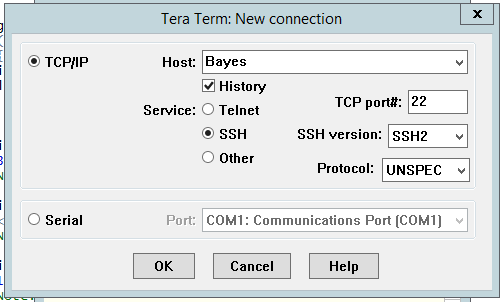
\includegraphics[width = .45\textwidth]{plots/tera_term_example.png}
\end{frame}

\begin{frame}
\frametitle{Using the cluster: logging in (Mac/Linux)}
\begin{enumerate}
\item Open a Terminal window
\item[]
\item Type \texttt{ssh mynetid@cluster.washington.edu}
\begin{itemize}
\item replace \texttt{mynetid} with Your UW NetID, and 
\item replace \texttt{cluster} with Your cluster, e.g., \texttt{bayes}
\end{itemize} 
\item[]
\item Enter password (same password as \texttt{box}) when prompted (the field will remain blank but your password will be received)
\end{enumerate}

\end{frame}

\begin{frame}
\frametitle{Using the cluster: logging in}
Your turn! Take 2 minutes to complete this activity \textbf{by yourself} (if you don't have a computer, write down how you would do this).
\begin{enumerate}
\item Log into the cluster
\item What is the name of the directory that you are when you log in?
\item Create a directory called \texttt{robust\_ses} in your \texttt{home} directory
\item Create a directory called \texttt{robust\_ses} on \textbf{your} computer, under \texttt{biost561/lecture9}
\end{enumerate}
\end{frame}

\begin{frame}
\frametitle{Using the cluster: moving around}
The cluster runs on Linux: in particular, the tools you learned in lecture 8, including \vspace{-0.3cm} \pause
\begin{itemize}
\item navigation, \pause
\item vim, \pause
\item commands, \pause and
\item shell scripts
\end{itemize}
are all used \textcolor{blue}{in exactly the same way}!
\end{frame}

\begin{frame}
\frametitle{Using the cluster: jobs}
The basic unit of cluster computing is a \textcolor{cyan}{job}. \pause

Jobs: \vspace{-0.3cm} \pause
\begin{itemize}
\item perform a specified task \pause
\item can be submitted to the cluster compute nodes \pause
\end{itemize}

Example job: run \texttt{run\_sim\_robust\_se.R} with 50 replicates
\end{frame}

\begin{frame}
\frametitle{Using the cluster: jobs}
\begin{center}
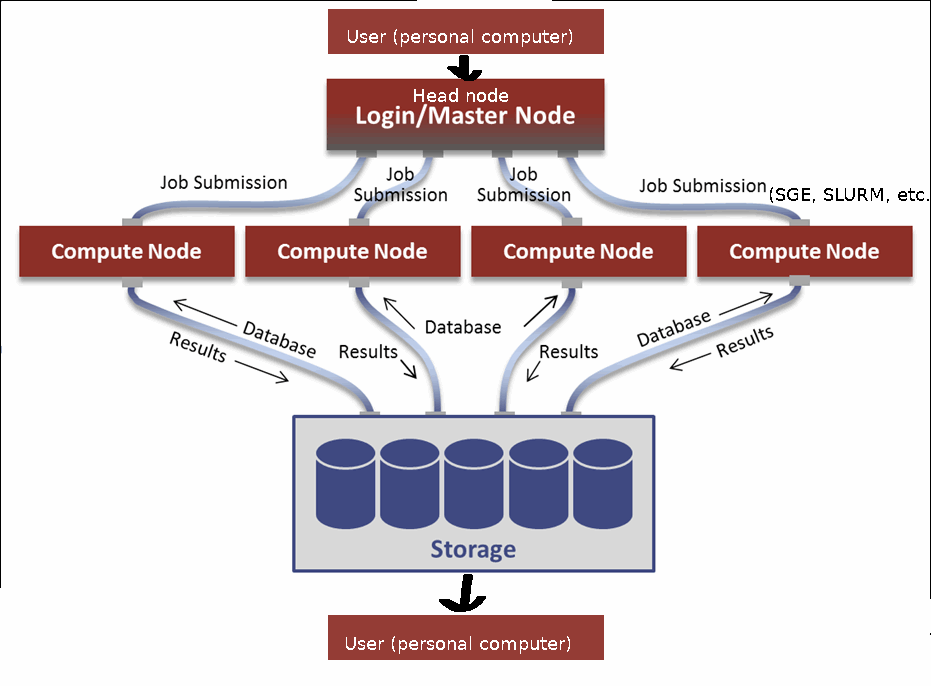
\includegraphics[width = 1\textwidth]{plots/hpc_system.png}
\end{center}
\end{frame}

\begin{frame}
\frametitle{Using the cluster: calling your \texttt{R} script}

Your turn!

Check out the file \texttt{call\_sim\_robust\_se.sh}. \textbf{With a partner}, answer the following questions: \vspace{-0.3cm}
\begin{enumerate}
\item What does the \texttt{\$} mean?
\item How many command-line arguments does \texttt{run\_sim\_robust\_se.R} take?
\item What do the command-line arguments do?
\end{enumerate}
\end{frame}

\begin{frame}
\frametitle{Using the cluster: submitting jobs}
Workhorse command on SGE: \href{http://gridscheduler.sourceforge.net/htmlman/htmlman1/qsub.html}{qsub}

Many options, including: \vspace{-0.3cm} \pause
\begin{itemize}
\item \texttt{cwd}: execute script in current working directory \pause
\item \texttt{e} and \texttt{o}: send error and output files to a folder, e.g., \texttt{iotrash/} \pause
\item \texttt{t <task1-taskn>} submits a job array with \texttt{taskn}$-$\texttt{task1} tasks \pause (more to come on this)
\end{itemize}

Options are specified with a single \texttt{-}, as you saw in Lecture 8.
\end{frame}

\begin{frame}
\frametitle{Using the cluster: job arrays}

Continuum of task types: \vspace{-0.3cm} \pause
\begin{itemize}
\item embarrassingly parallel: \pause can be split into sub-tasks run simultaneously \pause (e.g., sim with varying parameters)
\item inherently serial: \pause cannot be split into concurrent sub-tasks \pause (e.g., \texttt{run\_sim\_robust\_se.R} with one replicate per job) \pause
\end{itemize}

\textcolor{blue}{Job arrays} make embarrassingly parallel tasks easy: \vspace{-0.3cm} \pause
\begin{itemize}
\item unique identifier for an entire set of jobs \pause (easy to manage) \pause
\item unique identifier for each task within array \pause (set simulation parameters) \pause
\item displays nicely on cluster \pause (part of not flooding) 
\end{itemize}
\end{frame}

\begin{frame}
\frametitle{Using the cluster: batch submission scripts}

Your turn!

Check out the file \texttt{submit\_sim\_robust\_se.sh}. \textbf{With a partner}, answer the following questions: \vspace{-0.3cm}
\begin{enumerate}
\item What do lines 3 and 4 do? 
\item How many jobs are in my array if I want 5000 total jobs and 50 replicates per job?
\end{enumerate}

\end{frame}

\begin{frame}
\frametitle{Using the cluster: batch submission}

Your turn! 

Run the executable file \texttt{submit\_sim\_robust\_se.sh}, with command line arguments \vspace{-0.3cm}
\begin{itemize}
\item \texttt{"robust\_se"}
\item 5000
\item 50
\end{itemize}
\end{frame}

\begin{frame}[fragile]
\frametitle{Using the cluster: \texttt{simulator}}
\texttt{simulator} on the cluster: you have to grab nodes \textcolor{red}{manually}. \pause

Then, pass them as a character list into the argument \texttt{parallel}, e.g., \pause
\begin{verbatim}
list_of_names <- <get correct names>
simulate_from_model(nsim = 1000, 
       index = 1:3, 
       parallel = list(socket_names = list_of_names))
\end{verbatim} 

\end{frame}

\begin{frame}
\frametitle{Using the cluster: checking and altering jobs}

Many options once you have submitted a job: \vspace{-0.3cm} \pause
\begin{itemize}
\item \texttt{qstat} checks queue status; \vspace{-0.1cm} \pause helpful args:
\begin{itemize}
\item \texttt{f} shows full status of jobs
\item \texttt{u <user>} shows status only for \texttt{user} (e.g., \texttt{brianw26})
\item \texttt{j <jobnum>} shows details for a single job 
\end{itemize} \pause
\item \texttt{qhold <job\_id>[.tasklist]} puts a hold on job \texttt{job\_id} (and optionally array elements in \texttt{tasklist}) \pause
\item \texttt{qrls <job\_id>} removes a hold on a job
\item \texttt{qdel <job\_id>} deletes a job
\item \texttt{qalter <job\_id>} alters a job 
\end{itemize}
\end{frame}

\begin{frame}
\frametitle{Using the cluster: other helpful SGE commands}

Remember: \texttt{bayes} is a shared resource! \pause

Rule of thumb: \textcolor{ForestGreen}{20} jobs running on cluster at once. \pause

Ways to help share the cluster: \vspace{-0.3cm} \pause
\begin{itemize}
\item Submit batch jobs in job arrays \pause
\item Use holds on jobs, using \texttt{tc} argument in \texttt{qsub} \pause
\item Estimate timing of smallest job, consider this when creating and submitting job arrays
\end{itemize}
\end{frame}

\begin{frame}
\frametitle{Using the cluster: checking and altering jobs}

Your turn!

\begin{enumerate}
\item Check the status of \textbf{your} job array (replace my netid with yours): \texttt{qstat -f -u brianw26}
\item Allow only 20 jobs to run at a time (replace \texttt{<job\_id>} with your job id): \texttt{qalter <job\_id> -tc 20}
\end{enumerate}
\end{frame}

\begin{frame}
\frametitle{Using the cluster: wrapping up}
After all jobs are finished, pull results back to your machine. \pause

Then run your downstream code to compile results! \pause

Your turn! \vspace{-0.3cm}
\begin{enumerate}
\item Pull results files back to your computer
\item Run \texttt{load\_sim\_robust\_se.R}
\item What can you conclude based on these results?
\end{enumerate}
\end{frame}

\begin{frame}
\frametitle{Using the cluster: wrapping up}
Today, you practiced how to \vspace{-0.3cm} \pause
\begin{itemize}
\item run code without a GUI, \pause
\item use shell scripts, \pause
\item build a simulation, \pause
\item code modularly, \pause
\item and use the department cluster! \pause
\end{itemize}

These skills are easily portable to other cluster systems and your own coding projects (e.g., \texttt{R} packages). \pause

Remember to \textcolor{blue}{be nice}: the cluster is a shared resource!

\end{frame}

% section 3: appendix, other useful commands
\section*{Appendix: other useful cluster things}
\begin{frame}
\frametitle{}
\begin{center}
{\large \textbf{Appendix: other useful cluster things}}
\end{center}
\end{frame}
\begin{frame}
\frametitle{Useful things: Windows file compatability}
Editing files in Windows carries risks. 

One such risk is adding \textit{control characters} that cannot be processed on Unix systems (e.g., Linux on department cluster).

A helpful tool to remove this characters is \texttt{dos2unix}: to remove control characters from \texttt{myfile.sh}, run \texttt{dos2unix myfile.sh}.
\end{frame}

\begin{frame}[fragile]
\frametitle{Useful things: emails and other defaults}
You can set default behavior (on \texttt{bayes}, but similar for other systems) by creating a file called \texttt{.sge\_request}. 

Mine reads \vspace{-0.3cm}
\begin{verbatim}
-j y
-cwd
-S /bin/bash
-q normal.q
-M brianw26@uw.edu
-m e
\end{verbatim}

Which means: \vspace{-0.3cm}
\begin{itemize}
\item submit either binary or script file
\item run using \texttt{bash}
\item email me
\item email me at end of job
\end{itemize}
\end{frame}

\begin{frame}[fragile]
\frametitle{Useful things: aliases and functions (Mac/Linux)}
You will probably end up logging into the cluster or sending files back and forth \textcolor{blue}{quite often}.

Having \textit{aliases} and \textit{bash functions} set up makes this easier.

Creating aliases: \vspace{-0.3cm} 
\begin{enumerate}
\item go to your \texttt{.ssh} folder (in your home directory on your computer)
\item create a file called \texttt{config} (using, e.g., vim)
\item edit it using the template below
\end{enumerate} \vspace{-0.3cm}
{\scriptsize
\begin{verbatim}
Host <replace with, e.g., bayes>
    HostName <replace with, e.g., bayes.biostat.washington.edu>
    User <replace with, e.g., brianw26>
\end{verbatim}
}
\end{frame}

\begin{frame}[fragile]
\frametitle{Useful things: Useful things: aliases and functions (Mac/Linux)}
Creating functions: \vspace{-0.3cm} 
\begin{enumerate}
\item go to your home directory
\item create a file called, e.g., \texttt{.bash\_funcs}
\item edit it using the template below
\item edit your \texttt{.bashrc} file to include the lines \vspace{-0.1cm}
{\scriptsize
\begin{verbatim}
if [ -f ~/.bash_funcs ]; then
    . ~/.bash_funcs
fi
\end{verbatim}
}
(makes sure that \texttt{.bash\_funcs} is sourced when you open a new Terminal window)
\end{enumerate} \vspace{-0.3cm}
{\scriptsize
\begin{verbatim}
function_name () {
    commands
}
\end{verbatim}
}

E.g.~: send R files from cwd to specified directory on \texttt{bayes}: \vspace{-0.3cm}
{\scriptsize
\begin{verbatim}
send_r_bayes () {
    scp *.R brianw26@bayes.biostat.washington.edu:~/$1
}
\end{verbatim}
}
\end{frame}

\begin{frame}
\frametitle{Useful things: FileZilla (all, but esp. Windows)}
FileZilla is a nice program for pulling results back to your computer (via \texttt{scp}). 

It can be used on all types of computers, but is especially helpful for Windows (since command prompt is strange!).
\end{frame}

\end{document}
